\documentclass[11pt]{article}
\usepackage[alf]{abntex2cite}	% Citações padrão ABNT
\usepackage[utf8]{inputenc}     % 
\usepackage{graphicx}
\usepackage{xcolor}
\usepackage{lineno}
\linenumbers
\usepackage{ulem} % \sout - risca a linha
\usepackage{mathtools}
\usepackage{multirow}
\usepackage{multicol}
\usepackage{geometry}
 \geometry{
 a4paper,
 total={170mm,257mm},
 left=20mm,
 top=20mm,
 }

\title{FFLCH Libolo (Análise estatística)}
\author{Verónica Andrea González-López \\ Rafael Rodrigues de Moraes}
\date{Fevereiro 2021}

\begin{document}

\maketitle

\section{Statistical analyses}

Given the nature of the problem under investigation, in which the experimental units weren't selected probabilistically, all the following analyses and conclusions drawn by means of this \textit{observational study} cannot be generalized to populations other than the observed sample described at Section YY.

As described earlier in Section XX, the calling duration of a {\it{word}} was measured under two different settings, each representing a specific kind of calling, setting 1 ({\it{initial}}): calling without emphasis and setting 2 ({\it{insistent}}): calling with emphasis. Each speaker contributes with at least two replicates of the {\it{word Marina}} under both settings, {\it{initial}} and {\it{insistent}}.  
From the statistical point of view and formal terminology, one can describe this setup as the fairly common paired data comparison with replications. In the table \ref{tab:datastructure} we illustrate the data structure 

\begin{table}[h!]
 \caption{Illustration of the data structure for 2 speakers, speaker 1 with triplicates and speaker 2 with duplicates. $M_{ini}^{i,j}$ ($M_{insis}^{i,j}$) indicates the pronunciation of the word {\it{Marina}} under the setting {\it{initial}} ({\it{insistent}}) for the speaker $i$ and the replicate $j.$}
    \label{tab:datastructure}
    \centering
    \begin{tabular}{c|c|c}
        Speaker $i$ & {\it{Marina}} (initial) &{\it{Marina}} (insistent)  \\
        $i=1$ & $M_{ini}^{1,1}$ & $M_{ins}^{1,1}$\\
        $i=1$ & $M_{ini}^{1,2}$ & $M_{ins}^{1,2}$\\
        $i=1$ & $M_{ini}^{1,3}$ & $M_{ins}^{1,3}$\\ \hline
        $i=2$ & $M_{ini}^{2,1}$ & $M_{ins}^{2,1}$\\
        $i=2$ & $M_{ini}^{2,2}$ & $M_{ins}^{2,2}$
    \end{tabular}
\end{table}

The records of the duration are used to investigate whether the pronunciation {\it{insistent}} verifies a duration greater than the  modality {\it{initial}}. Such a situation will also be seen by syllables of the word, in order to identify in which syllable the modality produces a major impact. That is, for the syllables of the word, we have a similar structure to the one illustrated in table \ref{tab:datastructure}.

Although small in size and especially by taking advantage of the replications, the sample of $n=5$ participants produced in total 21 calling duration pairs for each syllable providing a valuable means for conducting an adequate exploratory data analysis which unveils the first visual pieces of evidence of a difference in calling durations for the two call types. 

Usually one proceeds to the visualization of the sample with the rather natural histogram, but due to the reduced sample size and our need for inspecting the sample avoiding any loss of visual information we opted for the dot plot, an adequate way of conveying visual information for relatively small data sets -- see \citeonline[Chapter 8]{ibe2014fundamentals} and \citeonline{cleveland1993visualizing}. Furthermore, as we are interested mainly in comparing the position of the distributions on the common scale of the calling duration in milliseconds, the dot plot is justified as an adequate choice according to \citeonline{cleveland1984graphical}.

\begin{figure}[ht]
    \centering
    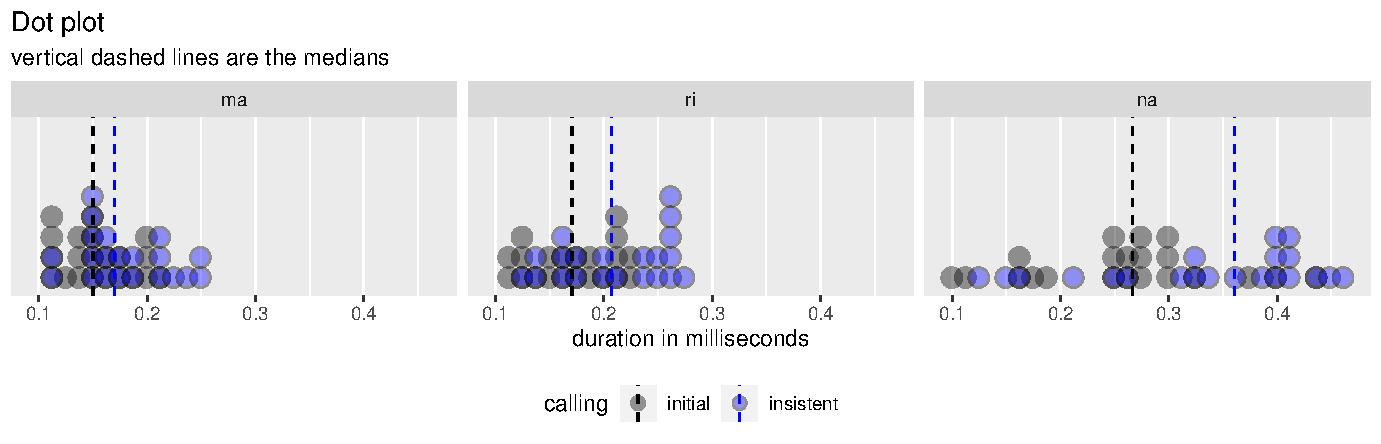
\includegraphics[width=1\textwidth]{dotplot.pdf}
    \caption{Exploratory data analysis of the distribution from calling durations.}\label{fig:dotplot_EDA}
\end{figure}

On figure \ref{fig:dotplot_EDA} one can note that for all syllables the insistent calling (in blue) is mainly right positioned in comparison with the initial calling (in grey), providing initial evidence of duration difference between the two settings. The variation appears to grow as one moves throughout the final syllables and because the duration of the individual syllables add-up to the duration of the whole word (Marina), its variation is the greatest on both types of calling. Furthermore, this exploratory data analysis naturally suggests the statistical techniques for verifying formally the significance of these differences, since it offers us support for the conjecture of longer duration associated with the {\it{insistent}} execution modality.

%\subsection{Null hypothesis significance testing (NHST)}

One can formally test the significance of these differences using either classic hypothesis tests (both parametric and nonparametric ones) or recent bayesian alternatives to those tests. Either way one has to work with the assumption of independent and identically distributed (iid) observations as the likelihood principle encompasses all those methods. As the replications present in the data set violate the independence assumption since it is not possible to consider independence between two replicates of the same speaker, to proceed with the tests we only used prototypical pronunciations (one by each speaker), indicated by experts.  Note further that we can reasonably assume independence between the participants, bringing down our sample size to $n=5.$

The standard hypothesis tests suitable for this situation are the parametric \textit{paired T-test} and its nonparametric counterpart \textit{Wilcoxon signed-rank test} (\citeonline{wilcoxon1992individual}). The T-Test requires normally distributed observations on both sets of the paired values, a probably stringent assumption for such a small sample size of $n=5$. Any strong deviation from normality implies in loss of test power or even the complete invalidation of its use. On the other hand, being distribution-free by not imposing any shape or structure in the original data, the Wilcoxon signed-rank test can be safely applied to paired differences when the assumption of normality is suspect (\citeonline[p. 590]{johnson2010statistics}). It basically assumes that the bivariate data are mutually independent, come from the same population and that the measurement scale is at least ordinal within each pair  (\citeonline{conover1998practical}).

As is often the case with nonparametric statistics, the Wilcoxon signed-rank test isn't based on the original data, but rather on its ranks.
Let $\left(X_i^{s}, Y_i^{s}\right)$ be the i-th paired observation, corresponding to the i-th speaker, where $X_i^{s}$ ($Y_i^{s}$) is the duration in milliseconds of the pronunciation of the syllable $s,$ under the setting {\it{initial}} ({\it{insistent}}), for $i=1,2,3,4,5$ and $s = \textrm{ma}, \textrm{ri}, \textrm{na}$. Also, define the sgn function, for any real number $x$, as $\textrm{sgn}(x) = 1$ if $x>0$, $\textrm{sgn}(x) = 0$ if $x=0$ and $\textrm{sgn}(x) = -1$ if $x<0$.


The hypothesis to be tested is $H_0$ (against $H_1$) where
\begin{itemize}
    \setlength{\itemindent}{4em}    
    \item[$H_0$:] The duration of the {\it{initial}} pronunciation is longer than the duration of the {\it{insistent}} one. 
    \item[$H_1$:] The duration of the {\it{initial}} pronunciation is shorter than the duration of the {\it{insistent}} one. 
\end{itemize}
This means, if we reject $H_0,$ the data shows a tendency in favor of $H_1$ and, in that case, the conjecture previously stated by the descriptive analysis will be considered well supported (with a small p-value).

%{\color{red} {\underline{Proposta para o texto em azul abaixo}}\\

The construction of the test statistic requires the computation of $W^+ = \sum_{i=1}^{5} d_i\cdot R_i^{s},$ where $R_i^{s} = \textrm{rank}\left( \left| D_i^{s} \right| \right),$ $D_i^{s} = X_i^{s} - Y_i^{s},$ $d_i = 1_{\left\{\textrm{sgn}\left(D_i^s \right)=1\right\}}$ and $1_{\left\{x\right\}}$ is the indicator function, defined as $1_{\left\{x\right\}}=1$ if $x$ is true, and $0$ otherwise, $|x|$ denotes the absolute value of $x,$ and  $\textrm{rank}\left( \left| D_i^{s} \right| \right)$ denotes the position of $|D_i^s|$ in relation with the other 4 values $|D_j^s|, j \neq i.$  
A complementary statistic can be computed $W^-$ which is the sum of the ranks of the negative differences $D_i^{s}$ with the property $W^+ + W^-=\frac{n(n+1)}{2}=15,$ since $n=5$ in this case. Table \ref{tab:case_ma} illustrates the results for $s=ma.$
%}

%{\color{blue}
%One then derives difference between the initial and insistent callings $D_i^{s} = X_i^{s} - Y_i^{s}$, its the sign as $d_i = 1_{\left\{\textrm{sgn}\left(D_i^s \right)=1\right\}}$ and ranks the absolute value of the difference as  $R_i^{s} = \textrm{rank}\left( \left| D_i^{s} \right| \right)$, where $1_{\left\{x\right\}}$ is the indicator function defined as $1_{\left\{x\right\}}=1$ if $x$ is true, and $0$ otherwise.

%The test statistic $W^+$ is the sum of the ranks of the positive differences $D_i^{s}$, given by $W^+ = \sum_{i=1}^{5} d_i\cdot R_i^{s}$. As a consistency check, $W^+ + W^{-}$ must equal $\frac{n(n+1)}{2}$ as we are adding up the ranks 1 through n, where $W^-$ is the sum of the ranks of the negative differences $D_i^{s}$.
%}
\begin{table}[!htb]
    \centering
    \footnotesize
        \caption{Wilcoxon signed-rank test calculation details for the syllable \textit{ma}.  }
    
    \begin{tabular}{c|ccccc}
        \hline
        $i$ (Speaker) & 
        1 {\tiny(DOMJ)} & % DOMJ
        2 {\tiny(FSBF)} & % FSBF
        3 {\tiny(JOAL)} & % JOAL
        4 {\tiny(JUJM)} & % JUJM
        5 {\tiny(MMEF)} \\ %MMEF
        \hline
        Initial calling $X_i^{ma}$ &
        0.1498 &
        0.1609 &
        0.1732 &
        0.2041 &
        0.1087 \\
        Insistent calling $Y_i^{ma}$ &
        0.1567 &
        0.2339 &
        0.2115 &
        0.2531 &
        0.1487 \\
        Absolute difference $\left| D_i^{ma} \right|$ & %D_i^{ma} = X_i^{ma} - Y_i^{ma}$ &
        0.0070 &
        0.0731 &
        0.0383 &
        0.0490 &
        0.0400 \\
        sign of $ D_i^{ma}$ &
        -- &
        -- &
        -- &
        -- &
        --  \\
        $d_i$ &
        0 &
        0 &
        0 &
        0 &
        0  \\
        $R_i^{ma}$ & %R_i^{ma} = \texttt{rank}\left( \left|D_i^{ma} \right|\right)$ &
        5 &
        1 &
        4 &
        2 & 
        3 \\
        \hline
        Test statistics &
        \multicolumn{5}{c}{$W^{+} = 0$ and $W^{-}=15$} 
         \\
        %\hline
    \end{tabular}
\label{tab:case_ma}
\end{table}

The test statistic is  $W^+ = 0$, since there are no pairs that verify $X_i^{ma} > Y_i^{ma},$ compare the lines 1 and 2 of table \ref{tab:case_ma}, always the first line records lower values than those registered in the second line. Then we have a strong tendency in the opposite sense of $H_0,$ which is confirmed with a p-value=0.03125 producing the rejection of $H_0$ in favour of $H_1.$ 

%The test statistic, defined as the sum of the ranks from positive differences by $W^+ = \sum_{i=1}^{5} d_i\cdot R_i^{ma}$, equals 0 for the observed sample as there are no pairs which verify $X_i^{ma} > Y_i^{ma}$. 

%Under the null hypothesis, we expect the distribution of differences to be symmetric around zero. Furthermore the positives and negatives should be randomly distributed among the ranks and under this assumption, it is possible to determine the exact probability of every possible outcome for $W^+$

As one can see on table xx containing the original data set, regardless of the syllable chosen, all values of the insistent calling superseed the values of the initial calling, implying $W^+ = 0$ for all three syllables {\it{ma}}, {\it{ri}} and {\it{na}}. The exact p-value related to this test statistic is 0.03125, calculated with the function \texttt{wilcox.test} in the statistical language \texttt{GNU R}. Then, consistently for all the syllables, the evidence is supporting $H_1.$

%{\color{magenta}podemos ver em conjunto o texto a seguir?. Penso que o ideal seria focar ma necessidade de um modelo e não na faltas dos testes.}

%{\color{blue}\textbf{De acordo}, conforme falamos hoje de tarde, retirei o parágrafo com a observação sobre a correção de bonferroni para um teste adicional de diferença entre variâncias. Vide o último parágrafo em azul como ponto de partida sugerido para discutirmos a conclusão dessa seção e abrindo a deixa para seção de análise bayesiana.}\\

Despite providing the p-value and the effect size, the null hypothesis significance test does not quantify the difference in duration of the syllables nor provides any analysis of the difference between variations in the two groups, which, as seen in the last section, is remarkable in our sample data, pointing out to the need of digging in and investigating this feature. 

%To formally test for difference of variation, one has to conduct an additional hypothesis test, resulting in the need to adapt the significance level, usually upon a Bonferroni correction to protect against the family-wise error rate (FWER), which considerably diminishes the intended significance level $\alpha$ (the probability of Type I error), leading possibly to different results than the ones presented in the NSHT above.

One way to address this issue is by constructing a model which also takes into account the variance structure, offering additional flexibility in the types of analyses. \citeonline{kruschke2013bayesian}  suggests tackling such problems under the framework of the bayesian hierarchical modelling (also known as \textit{multilevel modelling}) and using bayesian estimation, seen in details in the next section.

%\pagebreak

\subsection{Modeling the Settings {\it{initial}} and {\it{insistent}}}

The methods mentioned in the last section are based on the classical frequentist statistics, which treats the sample (observed) data as random and the parameters of the probability distribution which generates the data as fixed. This has implications, for instance, in the way we interpret the estimators, confidence intervals and the hypothesis tests. Furthermore, these tests are most reliable as the sample size gets bigger.

Bayesian statistics, on the other hand, treats the sample (observed) data as fixed and the parameters of the distribution which generates the data as random. By means of probability distributions associated with these parameters we represent our state of knowledge about the problem under study. 

Despite being a paradigm shift in the way we treat the data and the parameters, bayesian estimation works regardless of the sample size, but as its size gets bigger, usually, one comes to practically the same conclusions of the classical frequentist statistics. It is when the sample size is small, therefore departing from the stability of asymptotic methods, that the conclusions tend to diverge.

One quantifies the prior beliefs about the parameters in a probability distribution (known as \textit{prior distribution}), updates this belief with the likelihood using bayes rule to finally arrive at the posterior distribution of the parameters. 

Bayesian estimation can therefore be seen as a method of reallocating belief toward the parameter values that are consistent with the observed data, making heavy use of stochastic simulations arising from Markov Chain Monte Carlo (MCMC) methods which approximate the often analytically intractable posterior probability distributions of the parameters.

% referenciar melhor, pois é quase o texto original...
%{\color{red}\itshape By introducing an intuitive bayesian approach to the problem of comparison, the method proposed on \citeonline{kruschke2013bayesian} provides complete distributional information on means and variations of each calling type, revealing the relative credibility of every possible difference of means, every possible difference of standard deviations, and all possible effect sizes, based naturally on the sample data and the theorical formulation of the hierarchical model.}

Denote the observed sample data as $\{(X_i^s,Y_i^s)\}_{i=1}^5,$ where $s$ denotes a specific syllable ($s=ma, ri, na$), and the parameters $\mu_x, \sigma_x, \mu_y, \sigma_y, \nu$ to be estimated by bayesian inference.

%\begin{equation}
 %   \underbrace{p(\mu_x, \sigma_x, \mu_y, \sigma_y, \nu |\{X_i^s,Y_i^s\}_{i=1}^5)}_\text{posterior} 
 %   \propto 
 %   \underbrace{p(\{X_i^s,Y_i^s\}_{i=1}^5|\mu_x, \sigma_x, \mu_y, \sigma_y, \nu)}_\text{likelihood} \times \underbrace{p(\mu_x, \sigma_x, \mu_y, \sigma_y, \nu)}_\text{prior} %/ \underbrace{p(D)}_\text{evidence}
  %  \label{eq:full_bayes_model}
%\end{equation}

% prioris fundamentadas aqui: http://doingbayesiandataanalysis.blogspot.com/2015/04/informed-priors-for-bayesian-comparison.html
The mathematical formulation of the bayesian hierarchical model proposed on \citeonline{kruschke2013bayesian} is 
\begin{eqnarray}\label{verosim}
X^s_i \sim t(\mu_x, \sigma_x, \nu),\,\,\
Y^s_i \sim t(\mu_y, \sigma_y, \nu), \,\,\,i=1, 2, \ldots, 5.
\end{eqnarray}

Equation (\ref{verosim}) means that the duration under each setting, {\it{initial}} ($X^s_i$) and {\it{insistent}} ($Y^s_i$), follows the location-scale T distribution $t(\mu_x, \sigma_x, \nu)$ and $t(\mu_y, \sigma_y, \nu),$ respectively, as defined on \citeonline[p.507]{jackman2009bayesian}.

We then specify the prior distributions for each parameter $\mu_x, \sigma_x, \mu_y, \sigma_y, \nu$; they represent the prior knowledge about the parameters: 
\begin{eqnarray}\label{mus}
\mu_x,\mu_y \sim \textrm{Normal}(\bar{z}_m, 1000 s_{z}),
\end{eqnarray}
\begin{eqnarray}\label{sigmas}
\sigma_x,\sigma_y \sim \textrm{Uniform}(s_{z}/1000, s_{z} 1000),
\end{eqnarray}
\begin{eqnarray}\label{nu}
\nu \sim \textrm{Exponential}\left( \frac{1}{29} \right)+1,
\end{eqnarray}
where $\bar{z}_m$ is the sample mean and $s_z = \frac{1}{m-1} \sum_{i=1}^{m} (z_i-\bar{z}_m)^2$ is the standard deviation of the combined ($m=2n=2 \times 5=10$) observed sample of $\{z_i\}_{i=1}^{10},$ such that $z_i=X_i^s,$ for $i=1,...,5$ and $z_i=Y_i^s, $ for $i=6,...,10$ (also known as \textit{pooled data}), with the constraint on the normality parameter $\nu\geq 1$. 

The priors, equations (\ref{mus}), (\ref{sigmas}), (\ref{nu}), are set to be very broad and vague in order for it to have minimal influence on the estimation, enabling the data to dominate the posterior distributions. 

The fact that the random vector $(X_i^s, Y_i^s)$ is assumed to follow the location-scale T distribution has little to do with their symmetry or shape. That distribution has more heavy tails than the normal distribution, and it is chosen in order to allow for robustness against outliers.

We have two scenarios, (i) {\it{initial}} and (ii) {\it{insistent}}, under which we must describe the performance of the {\it{duration}} in the pronunciation of each syllable of the word {\it{Marina}}. Each pronunciation under the two settings is represented by posterior distributions built through equations (\ref{verosim}) to (\ref{nu}). Under (i)  the process is represented by the posterior distributions of $\mu_x,$ $\sigma_x$ (subscript $x$) and $\nu,$ and under (ii) the process is represented by $\mu_y,$ $\sigma_y$ (subscripts $y$) and $\nu.$  

For a fixed syllable $s,$ under (i) (or (ii)), $\mu_x$ (or $\mu_y$) represents the performance of the central position of the duration of the pronunciation generating the syllable $s$, while $\sigma_x$ (or $\sigma_y$) represents the dispersion (variability) of the duration, which occurs during the pronunciation of the syllable $s$. In complement $\nu$ represents the degrees of freedom which is common for both (i) and (ii). $\mu_x, \sigma_x, \mu_y, \sigma_y, \nu$ under the bayesian perspective are random, following posterior distributions that need to be obtained by simulations. The posterior distributions incorporate information from the collected data. Then, in general lines, the posterior distributions are a consequence of the effect of the data. By inspecting such as distributions we can reveal characteristics of (i) and (ii); that is the goal here. 

As already stated, the response that the bayesian model offers is a portrait of the performance of both modalities (i) and (ii), by means of posterior distributions (for each one of the values $\mu_x, \sigma_x, \mu_y, \sigma_y$ and $\nu$ we obtain a posterior distribution). Each posterior distribution can be described by some list of values (see \citeonline{Robert2007}): (1) the {\it{mean}} (which is the bayesian point estimator under quadratic loss function), (2) the {\it{median}} (bayesian point estimator under absolute value loss function), (2) standard deviation ({\it{sd}}) that offers an indicator of the variability of the distribution, (3) $\mbox{HDI}_{\mbox{lower}},$ which is the lower limit of the credibility region and (4) $\mbox{HDI}_{\mbox{upper}},$ which is the upper limit of the credibility region. All of these indicators summarize the performance of the distribution and provide the basis for an analysis of the representation of (i) and (ii).
 The table \ref{tab:mcmc_results} reports the summaries of the posterior distributions of $\mu_x, \mu_y, \sigma_x, \sigma_y$ and $\nu,$ obtained by combining the equations (\ref{verosim}) to (\ref{nu}), for each syllable $s=$ ma, ri, na.  
 
 For each distribution, several Markov chains are simulated in order to achieve the convergence of the process, which is necessary to guarantee that we are describing the desired posterior distribution, see \citeonline{Robert2007}. All the distributions show evidence of convergence according to the eighth column of table \ref{tab:mcmc_results}, which records the coefficient $\widehat{R}$ ({\it{Brooks-Gelman-Rubin  scale  reduction  factor}}), see \citeonline{gelman2011inference}, which is 1 on convergence. The last column of table \ref{tab:mcmc_results} reports $n_{\text{eff}}$, the effective sample size, one measure of chain length which takes into account the known side-effect of autocorrelation when generating the markov chains. According to \citeonline{kruschke2014doing}, in order to compute credibility regions, given by the HDI values in table \ref{tab:mcmc_results} one needs a $n_{\text{eff}}$ of at least 10m000 samples which justifies the choice of 300 thousand total simulations for this study. 
 %The value of $n_{\text{eff}}$ reported in each case of table \ref{tab:mcmc_results} is convenient to define an adequate region of credibility (see \cite{kruschke2013bayesian}).
 
%{\color{red}
%\textbf{Pendências} (revistas após nossa conversa por videoconferência no sábado 27.02.2021 às 14h):
%
%\begin{enumerate}
%    \item a quest\~{a}o das unidades: $\mu$ e $\sigma$ milisegundos, para $\nu$ n\~{a}o sei.... \textcolor{blue}{\textbf{Rafael:} a unidade para $\sigma$ é millisegundos também. o rótulo do eixo x nos gráficos de $\nu$ estava errado no gráfico mesmo, agora eu corrigi - veja a figura \ref{fig:histograms_nu_mcmc}. Ele é o parâmetro de normalidade e seus valores não pertencem a nenhuma unidade mensurável como segundos, metros, etc... Sugiro deixar o rótulo sem texto e podemos explicar isso no rótulo da figura que vai no pdf. }
%    \item unificamos a descritiva e o teste? \textcolor{blue}{\textbf{Rafael:} vamos falar em breve, pois não entendo a pergunta... }
%\end{enumerate}

%}


\begin{table}[ht]
\centering
\footnotesize
\caption{Mean, sd, median, $\textrm{HDI}_{\text{lower}}$ and $\textrm{HDI}_{\text{upper}}$ (both at 95\%), $\widehat{R}$ and $n_{\text{eff}}$ from the posterior distribution for each parameter $\mu_x, \sigma_x, \mu_y, \sigma_y, \nu$ and for each syllable: ma, ri, na. }
\begin{tabular}{ccrrrrrrr}
  \hline
syllable & parameter & mean & sd & median & $\textrm{HDI}_{\text{lower}}$ & $\textrm{HDI}_{\text{upper}}$ & $\widehat{R}$ & $n_{\text{eff}}$ \\ 
	  \hline
	\multirow{5}{*}{ma} & $\mu_x$ & 0.1595 & 0.0299 & 0.1596 & 0.1033 & 0.2156 & 1.0010 & 60968 \\ 
	   & $\mu_y$ & 0.2012 & 0.0396 & 0.2012 & 0.1251 & 0.2768 & 1.0010 & 63439 \\ 
	   & $\nu$ & 33.0728 & 29.3461 & 24.4707 & 1.0013 & 91.3661 & 1.0000 & 63264 \\ 
	   & $\sigma_x$ & 0.0534 & 0.0395 & 0.0434 & 0.0140 & 0.1160 & 1.0010 & 15719 \\ 
	   & $\sigma_y$ & 0.0726 & 0.0540 & 0.0592 & 0.0214 & 0.1573 & 1.0030 & 13272 \\ 
	   \hline
	\multirow{5}{*}{ri} & $\mu_x$ & 0.1726 & 0.0398 & 0.1723 & 0.0984 & 0.2472 & 1.0010 & 53800 \\ 
	   & $\mu_y$ & 0.2224 & 0.0455 & 0.2228 & 0.1345 & 0.3098 & 1.0000 & 76452 \\ 
	   & $\nu$ & 33.8492 & 29.6130 & 25.2469 & 1.0013 & 92.8353 & 1.0000 & 61465 \\ 
	   & $\sigma_x$ & 0.0710 & 0.0510 & 0.0579 & 0.0209 & 0.1541 & 1.0040 & 15553 \\ 
	   & $\sigma_y$ & 0.0844 & 0.0572 & 0.0693 & 0.0254 & 0.1834 & 1.0030 & 20099 \\ 
	   \hline
	\multirow{5}{*}{na} & $\mu_x$ & 0.2770 & 0.0721 & 0.2770 & 0.1406 & 0.4174 & 1.0010 & 64643 \\ 
	   & $\mu_y$ & 0.3278 & 0.0758 & 0.3284 & 0.1862 & 0.4701 & 1.0000 & 57832 \\ 
	   & $\nu$ & 33.0314 & 29.4438 & 24.3532 & 1.0003 & 91.6137 & 1.0000 & 59973 \\ 
	   & $\sigma_x$ & 0.1327 & 0.0944 & 0.1085 & 0.0362 & 0.2896 & 1.0110 & 16361 \\ 
	   & $\sigma_y$ & 0.1372 & 0.0973 & 0.1124 & 0.0396 & 0.2953 & 1.0060 & 16151 \\ 
	   \hline
\end{tabular}
\label{tab:mcmc_results}
\end{table}

\begin{figure}[h!]
    \centering
    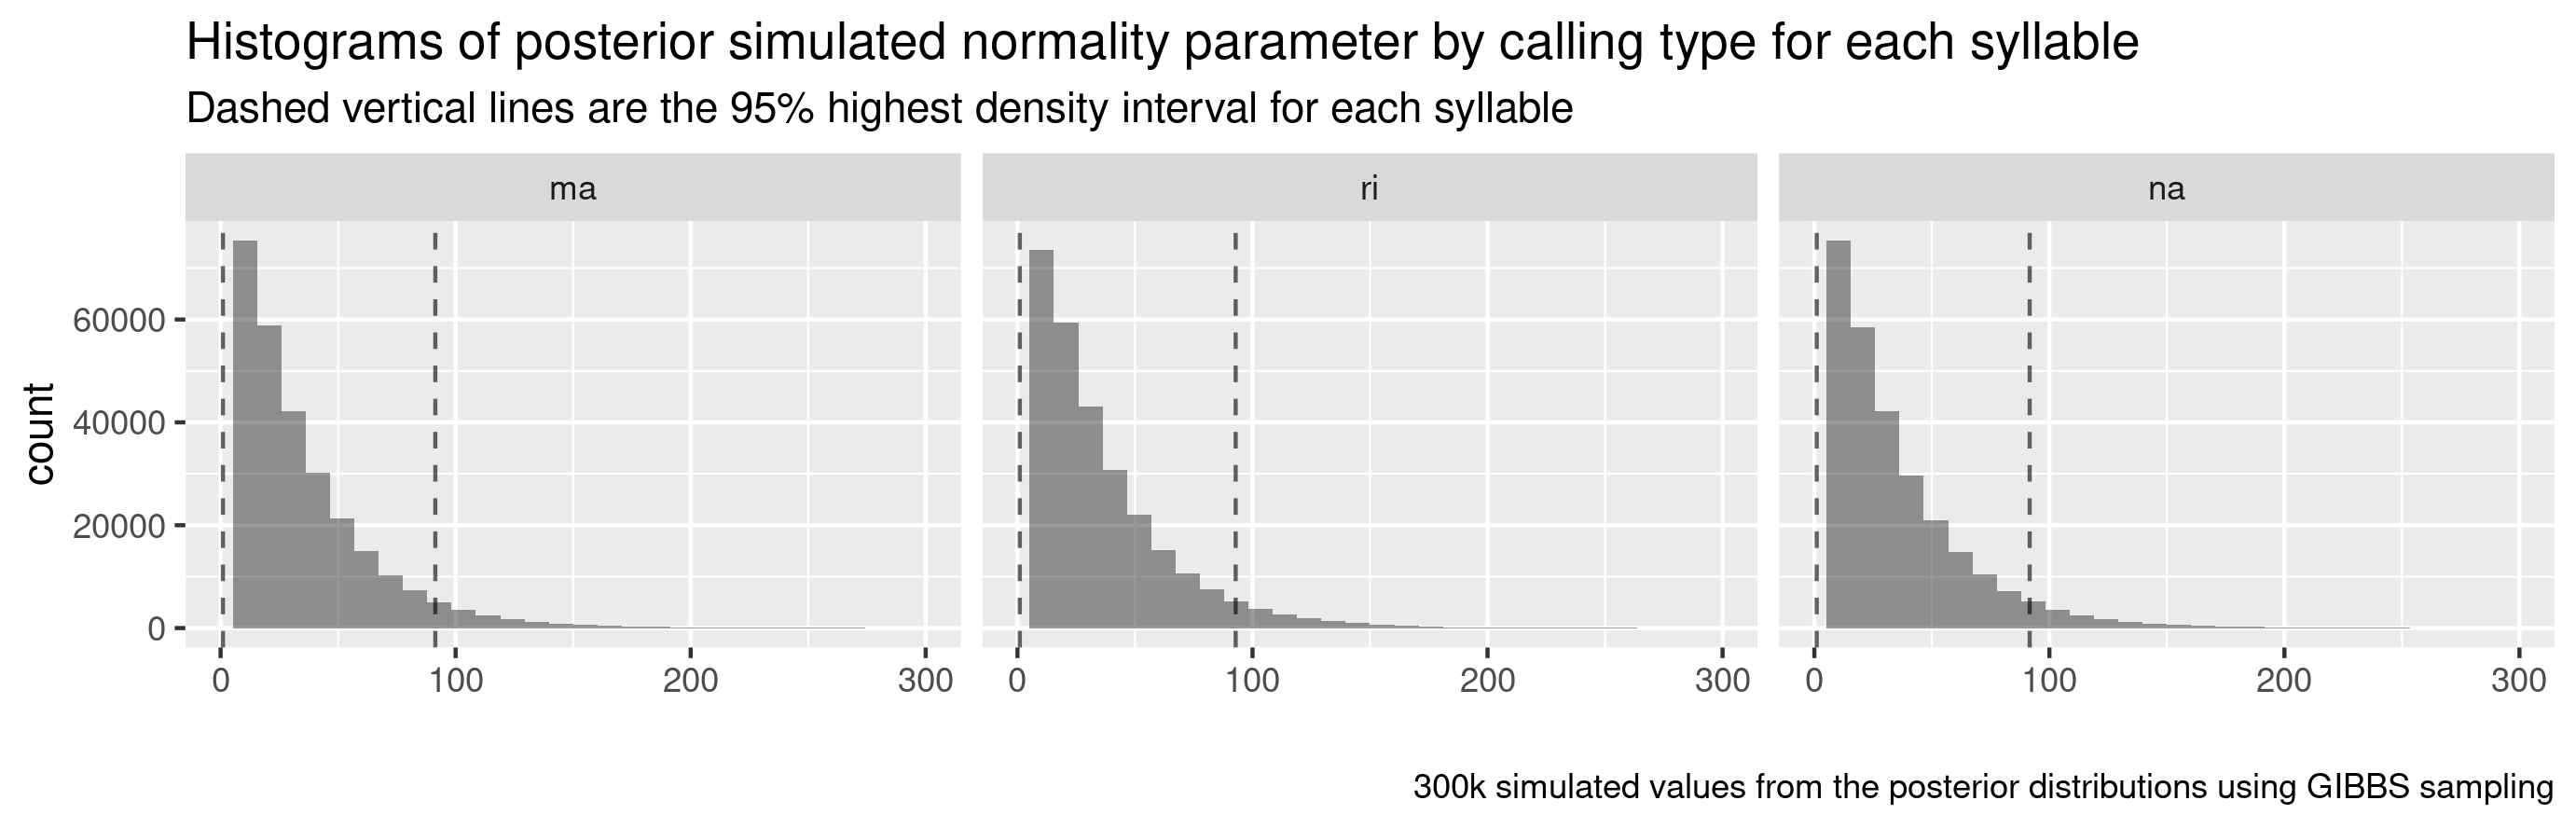
\includegraphics[width=1\textwidth]{histograms_nu.pdf}
    \caption{Histograms of the simulated posterior values of normality parameter $\nu$ (in grey) for each syllable: ma, ri, na. In vertical dotted lines, the lower ($\mbox{HDI}_{\mbox{lower}}$) and upper ($\mbox{HDI}_{\mbox{upper}}$) limits of the credibility regions (95\%).}
    \label{fig:histograms_nu_mcmc}
\end{figure}


Table \ref{tab:mcmc_results} and figure \ref{fig:histograms_nu_mcmc} show the evolution of the distribution of $\nu$ when running the syllables from {\it{ma}} to {\it{na}}. We notice a very similar behaviour when comparing the three distributions (one for each syllable), all three providing an estimated value $\nu$ which enables us to say that the adopted likelihood (see equation (\ref{verosim})) makes sense when comparing it with the normal likelihood (Gaussian). Generally the T distribution is close to the standard normal when its degrees of freedom are high. 

The posterior estimated mean value of $\nu$ (under quadratic loss function) for each syllable is moderate and approximately 33 (see mean value associated with $\nu$ in table \ref{tab:mcmc_results}). Note that as $\nu$ grows, both $X_i^s$ and $Y_i^s$ tend to the normal distribution and observing the curves in figure \ref{fig:histograms_nu_mcmc} we see that there are few possibilities that the value of $\nu$ exceeds 100. Even more, the upper end $\mbox{HDI}_{\mbox{upper}}$ of the 95 \% credibility regions in none of the 3 cases exceeds 93.

As we can see in table \ref{tab:mcmc_results}, both values, the mean and the median of $\mu_x$ and $\mu_y$ show that the estimation is greater in the {\it{insistent}} setting in comparison with the {\it{initial}} setting. For example for the syllable ma, we obtain, 
$\mbox{mean}(\mu_y)=0.2012>\mbox{mean}(\mu_x)=0.1595 \,\,\mbox{and}\,\, \mbox{median}(\mu_y)=0.2012>\mbox{median}(\mu_x)=0.1596.$ And, the relationships mean($\mu_y$)$>$mean($\mu_x$) and median($\mu_y$)$>$median($\mu_x$) are verified for all the syllables $s=$ ma, ri, na. 
This fact is also confirmed by the histograms of the values of $\mu_x$ (in grey) and $\mu_y$ (in blue) exposed in figure \ref{fig:histograms_mus_mcmc}, for each syllable. Note that the histograms in blue are always to the right of the histograms in gray. 

From figure \ref{fig:histograms_mus_mcmc} we obtain the relevant observation that, the posterior distributions reflect the variability of the original data, as the variance gets bigger when one moves through the final syllable of {\it{Marina}}. {\color{blue} Vinicius tem uma boa explica\c c\~{a}o para isto}. Each distribution (like those shown in figure \ref{fig:histograms_mus_mcmc}) has an area equal to 1 (equivalent to 100\%). We see then that the histograms with the highest modes distribute less mass to the right and to the left of them on the abscissa axis (axis-x), in other words, they are more precise regarding the concentration value. 

In view of this, the mean duration curves for each syllable are more precise or concentrated in the case of setting (i) when compared with the setting (ii), which shows less precision. This characteristic is evidenced in table \ref{tab:mcmc_results} by the relations $\text{sd}(\mu_y)> \text{sd}(\mu_x)$. For instance, for the syllable ma, we observe $\text{sd}(\mu_y)=0.0396>\text{sd}(\mu_x)=0.0299$.

The highest density regions $[\mbox{HDI}_{\mbox{lower}},\mbox{HDI}_{\mbox{upper}}]$ at 95\% level, which are those regions where the average duration values tend to occur, are reported in table \ref{tab:mcmc_results} and indicated in figure \ref{fig:histograms_mus_mcmc}. For instance, in the case of the syllable ma, those are $[0.1013,0.2156]$ for $\mu_x$ and $[0.1251,0.2768]$ for $\mu_y,$ both intervals display in the duration line (axis x) of figure \ref{fig:histograms_mus_mcmc} (on the left - case: ma).  The regions are delimited by vertical lines in blue (setting (ii)) and in grey (setting (i)). The regions of (ii) are always arranged to the right in relation to the regions of (i), this finding confirms once again the tendency of the setting (ii) ({\it{insistent}}) to produce durations with larger values in comparison with the setting (i) ({\it{initial}}).

The quantity $\sigma_x$ (or $\sigma_y$) represents the variability of the duration during the pronunciation of the syllable. With this in mind, note that the histograms of the values of $\sigma_x$ (in grey) and $\sigma_y$ (in blue) exposed in figure \ref{fig:histograms_sigmas_mcmc}, for each syllable, conveys also an analysis of the variation quantified formally, which get bigger as one moves from syllable \textit{ma} toward \textit{na}. Note that if you look at table \ref{tab:meanandsd} (values extracted from table \ref{tab:mcmc_results}) from top to bottom, by setting ((i) or (ii)), the mean and sd values increase. In other words, this evolution occurs independently of the setting. Then, the aspect that we want to reveal is how this variability occurs in each setting. 

\begin{table}[h!]
    \centering
     \caption{Mean and standard deviation of the posterior distributions of $\sigma_x$ and $\sigma_y.$}
    \label{tab:meanandsd}
    \begin{tabular}{c|cc||cc}
    & mean($\sigma_x$) & sd($\sigma_x$) & mean($\sigma_y$) & sd($\sigma_y$)\\ \hline
        ma & 0.0534 & 0.0395 &0.0726 & 0.0540 \\
        ri & 0.0710 & 0.0510 &0.0844 & 0.0572 \\
        na & 0.1327 & 0.0944 & 0.1372 & 0.0973
    \end{tabular}
\end{table}

We note that the histograms in figure \ref{fig:histograms_sigmas_mcmc} show greater precision in the case of setting (i) {\it{initial}} in comparison with the setting (ii) {\it{insistent}} (the curves in grey are higher). Such precision is reflected in a smaller amplitude of the credibility regions in the case of the curves in gray when compared with the curves in blue, this occurs in the 3 syllables and to a lesser degree in the last syllable of the word. Such information can be also found in table \ref{tab:mcmc_results}. For instance, if we focus on the syllable ma, we obtain $\mbox{mean}(\sigma_y)=0.0726>\mbox{mean}(\sigma_x)=0.0534,$ then we expect an inferior variability of duration when one pronounces such syllable under the setting (i) in comparison with the variability expected under the setting (ii).

\begin{figure}[!htb]
    \centering
    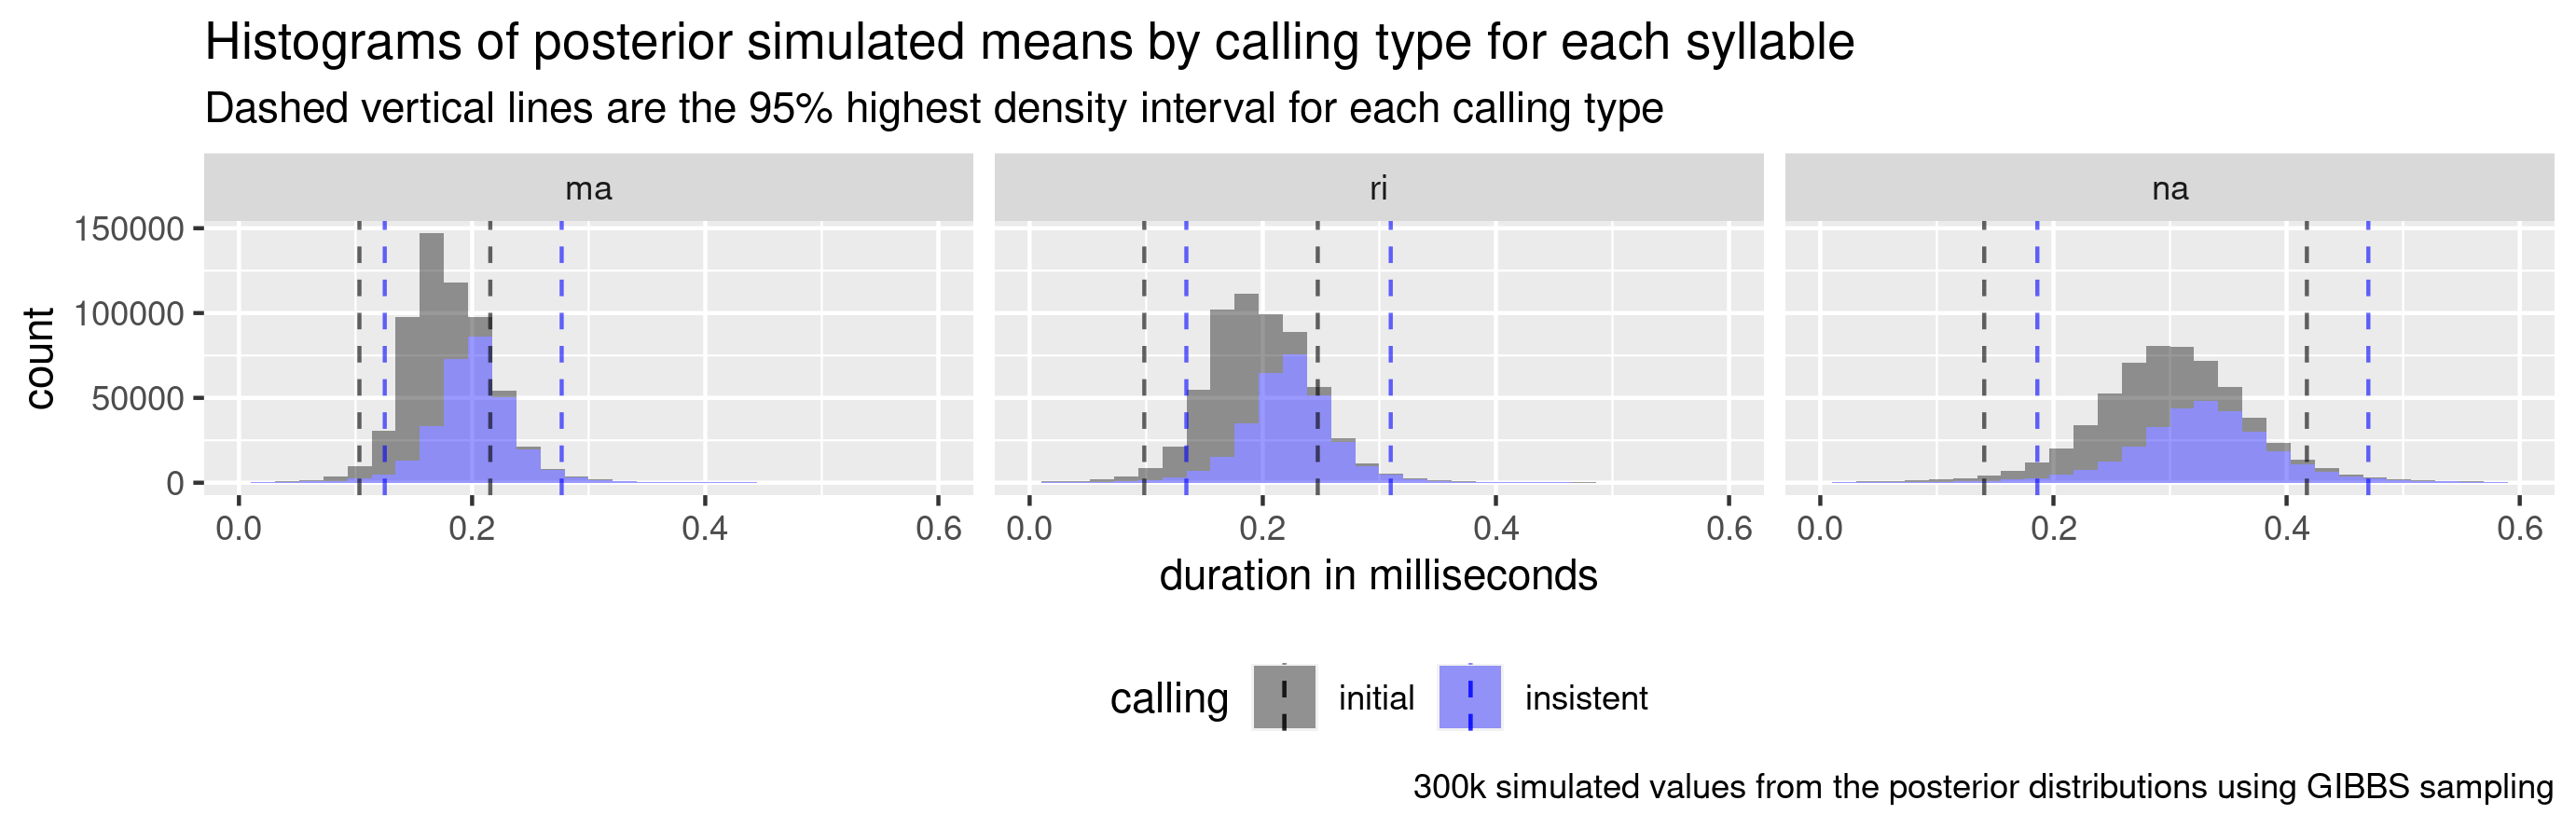
\includegraphics[width=1\textwidth]{histograms_mus.pdf}
    \caption{Histograms of the simulated posterior values of $\mu_x$ (in grey) and $\mu_y$ (in blue) for each syllable: ma, ri, na. In vertical dotted lines, the lower ($\mbox{HDI}_{\mbox{lower}}$) and upper ($\mbox{HDI}_{\mbox{upper}}$) limits of the credibility regions (95\%), for $\mu_x$ (in grey) and for $\mu_y$ (in blue).}
    \label{fig:histograms_mus_mcmc}
\end{figure}

\vspace{15mm}

\begin{figure}[!htb]
    \centering
    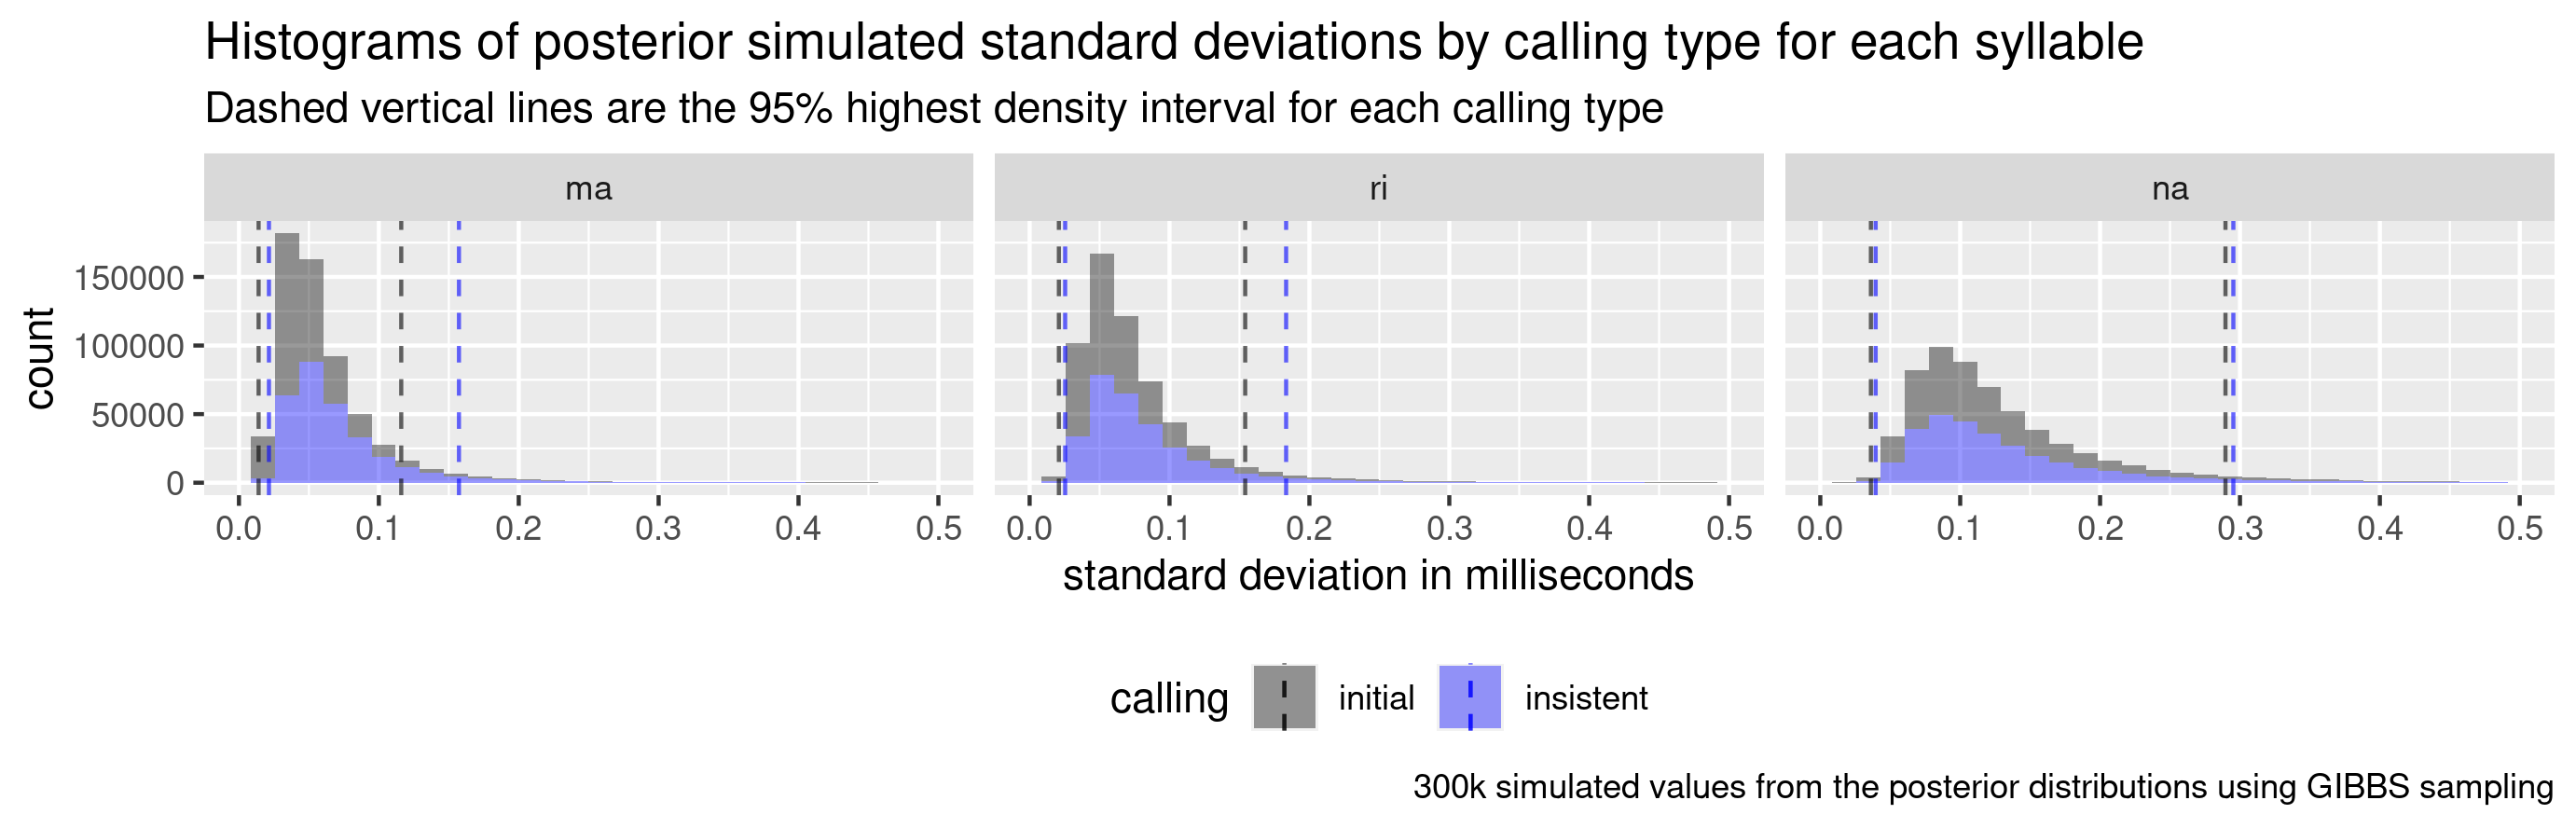
\includegraphics[width=1\textwidth]{histograms_sigmas.pdf}
    \caption{Histograms of the simulated posterior values of $\sigma_x$ (in grey) and $\sigma_y$ (in blue) for each syllable: ma, ri, na. In vertical dotted lines, the lower ($\mbox{HDI}_{\mbox{lower}}$) and upper ($\mbox{HDI}_{\mbox{upper}}$) limits of the credibility regions (95\%), for $\sigma_x$ (in grey) and for $\sigma_y$ (in blue).}
    \label{fig:histograms_sigmas_mcmc}
\end{figure}

\vspace{15mm}




%\pagebreak
%\subsection*{Appendix}

%\begin{figure}[!htb]
%    \centering
%    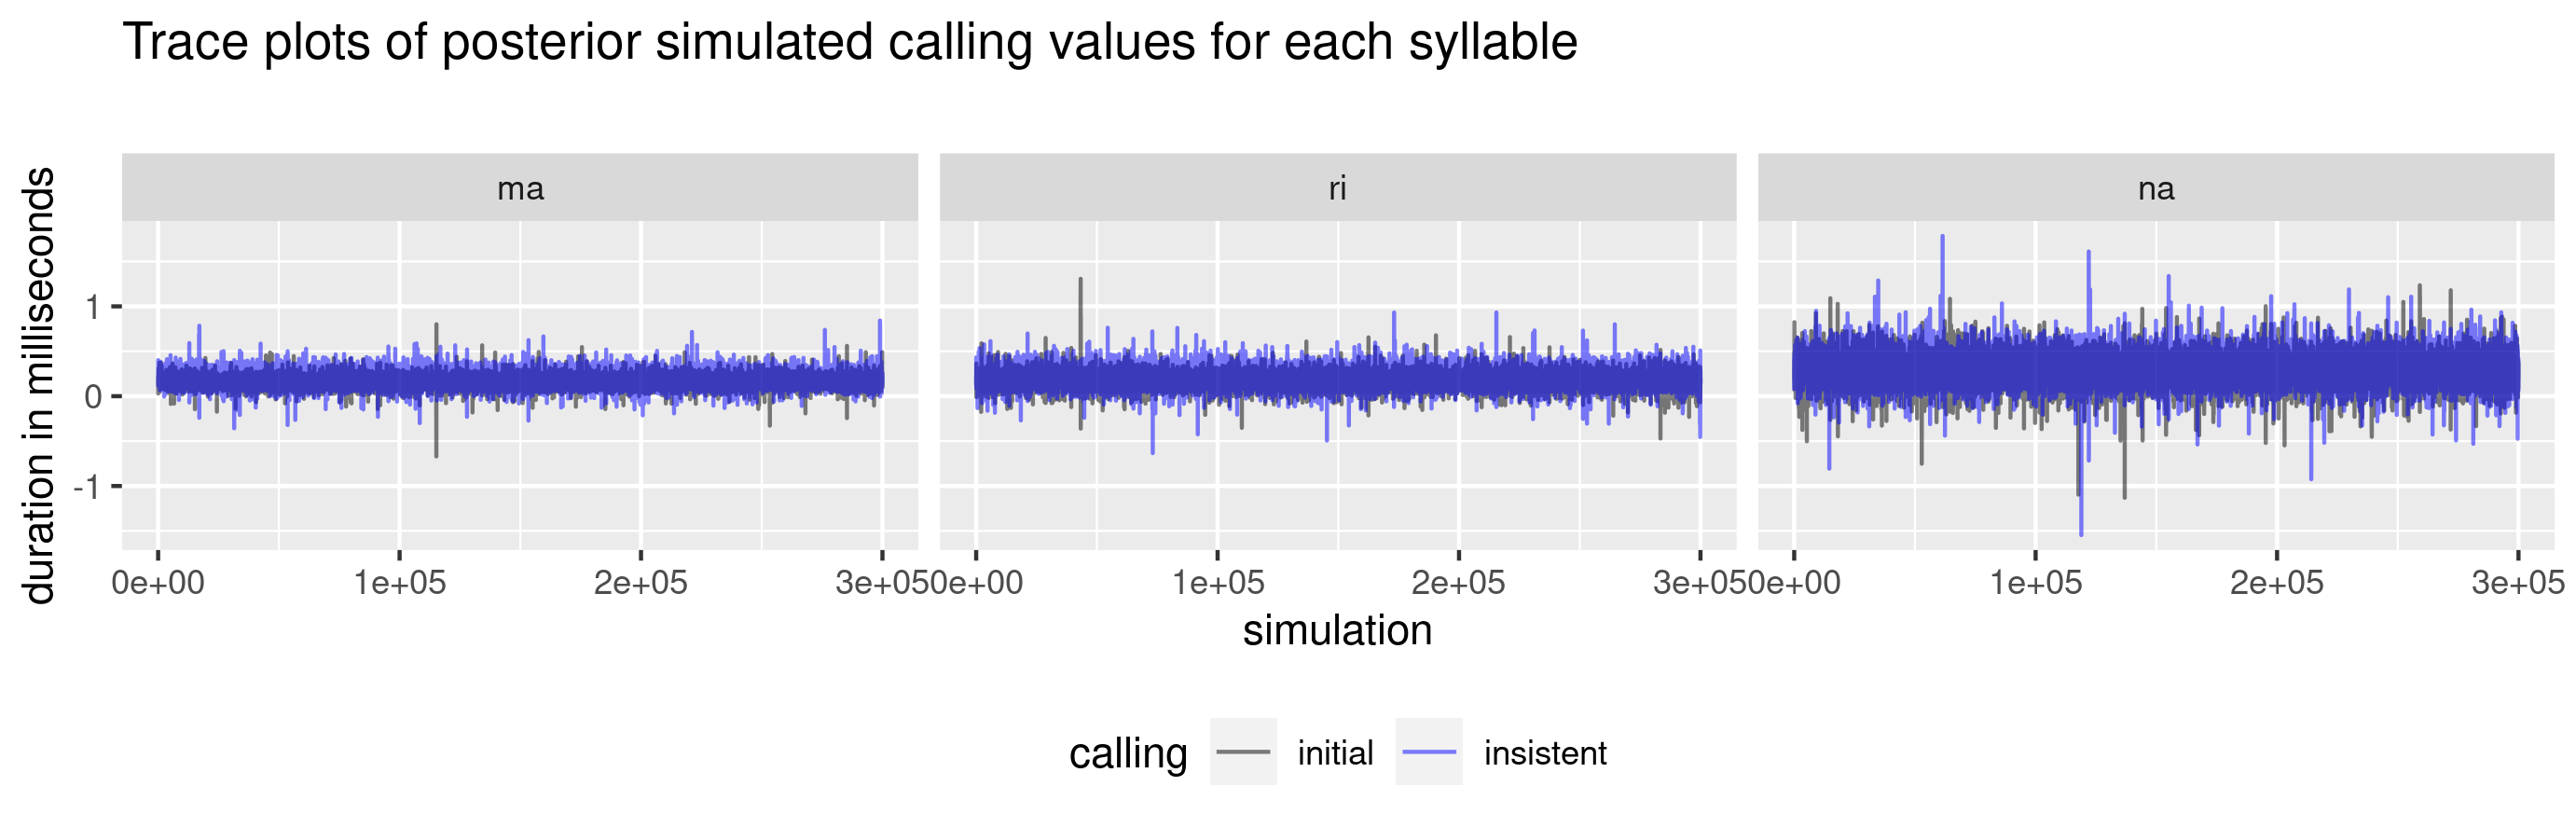
\includegraphics[width=1\textwidth]{traceplots.pdf}
%    \caption{Trace plots of the MCMC simulated posterior distribution of calling durations for each syllable. All six chains show evidence of convergence. Note further that the posterior distributions reflect the variability of the original data, as the variance gets bigger when one moves through the final syllable.}
%    \label{fig:traceplots_mcmc}
%\end{figure}

%\begin{figure}[!htb]
%    \centering
%    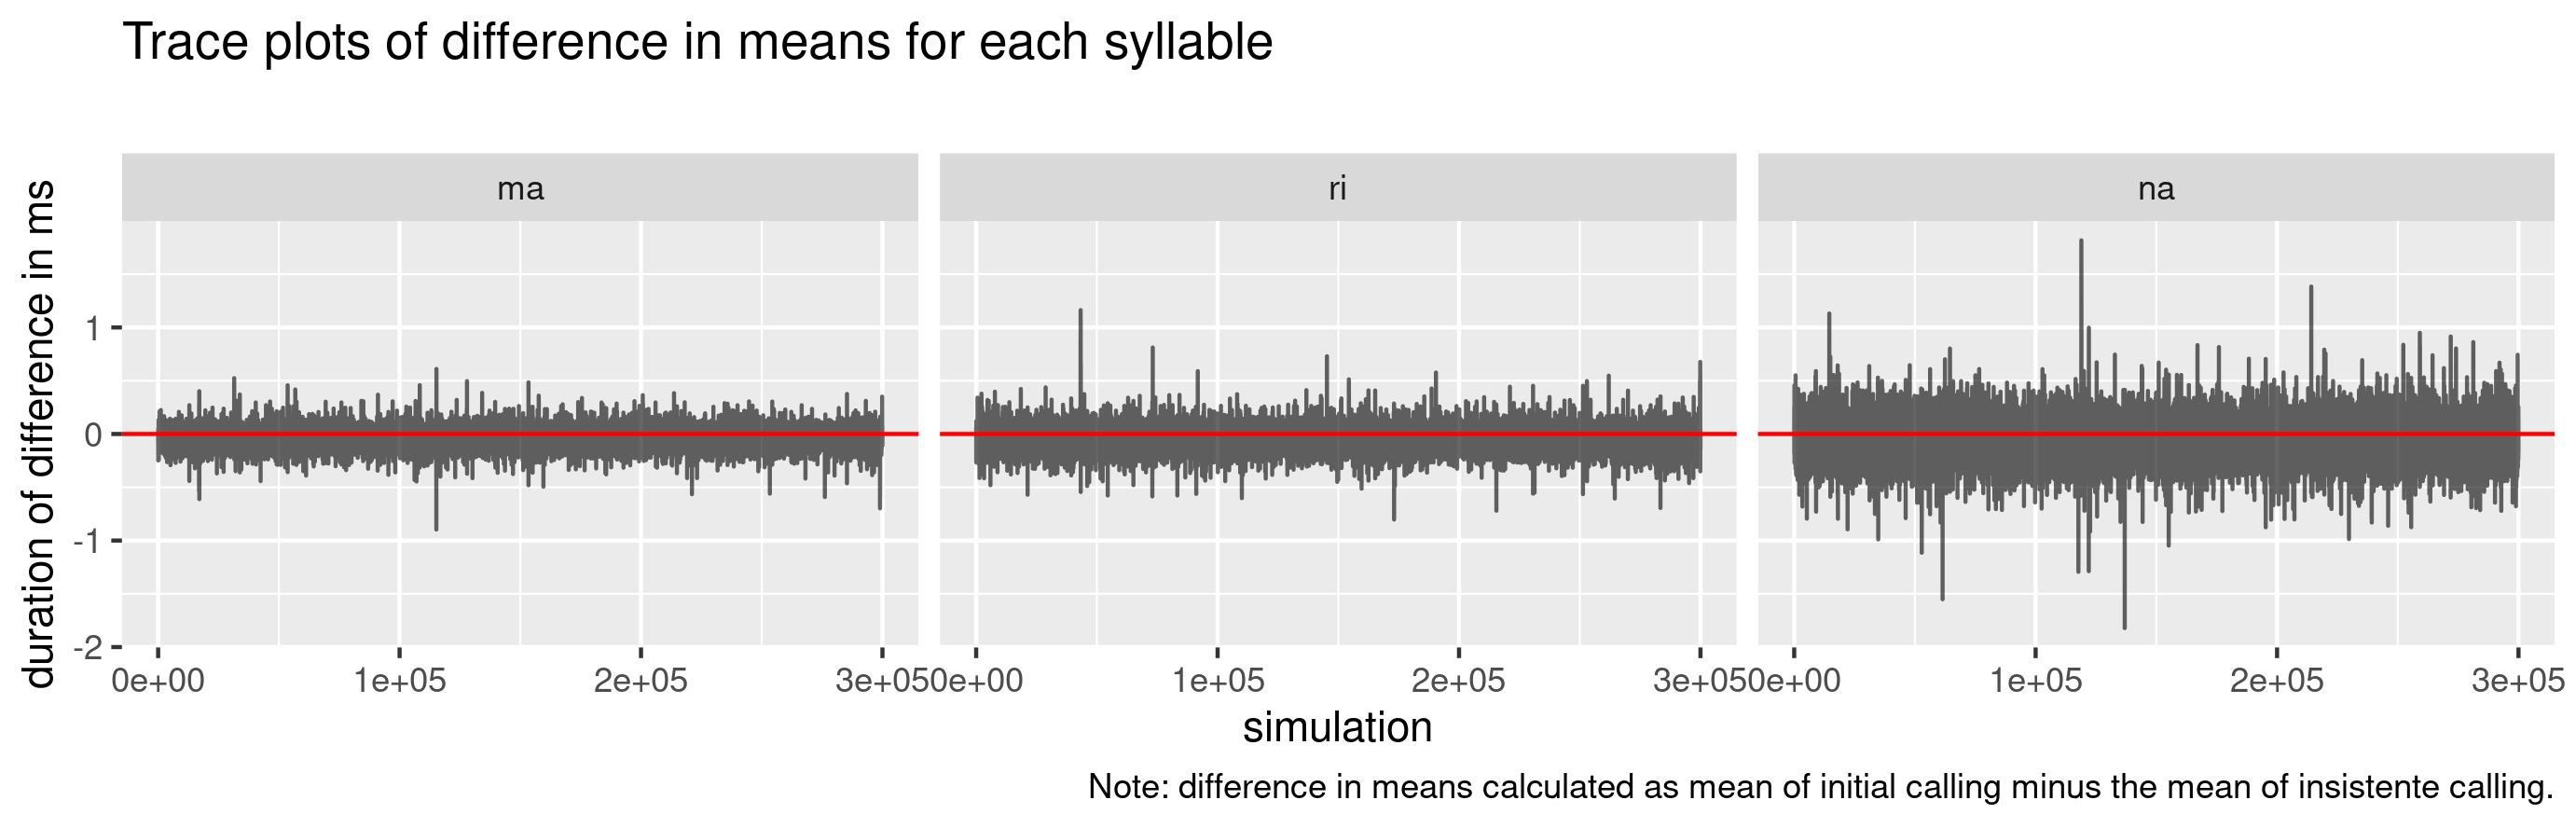
\includegraphics[width=1\textwidth]{traceplots_diffs.pdf}
%    \caption{Trace plots of the MCMC simulated posterior distribution of the differences in mean from calling durations for each syllable. Note that the differences reflect the variability of the original data, as the variance gets bigger when one moves through the final syllable.}
%    \label{fig:traceplots_diffs_mcmc}
%\end{figure}

\pagebreak
%\bibliographystyle{plain}
\bibliography{references}
\end{document}
